%\documentclass[MTRX3700report.tex]{subfiles}
\documentclass[11pt,a4paper]{article}
% Dpak
% HARDWARE DESIGN Appendix
\usepackage{color}
\usepackage{caption}
\usepackage{graphics}
\usepackage{graphicx}


\begin{document}
\title{Appendix A: Hardware Connections}
\maketitle

\section{Mobile Robot}
\subsection{Power Board}
  \label{appA:Power Board}
  The following tables are the pin connectors located on the power board. Connectors X2, X3 and X5 are connected internally to the Pololu Hbridge motor driver circuit, and all inputs to the motor drivers are instead connected to the power board.
  \\
  \begin{table}[h!]
    \flushleft

    \begin{minipage}{0.45\textwidth}
      \begin{tabular}[b]{|p{7mm}|p{4.5cm}|}
        \hline \textbf{Pin} & \textbf{Signal}\\
        \hline 1 & +11 V to +20.0 V Input\\
        \hline 2 & +0.0 V Ground\\
        \hline
      \end{tabular}
      \caption{Connector X1}
      \vspace{25pt}
    \end{minipage}\hfill
    \begin{minipage}{0.45\textwidth}
      \begin{tabular}[b]{|p{7mm}|p{4.5cm}|}
        \hline \textbf{Pin} & \textbf{Signal}\\
        \hline  1 & +5 V Supply to Encoder 1\\
        \hline  2 & Encoder 1 A Output\\
        \hline  3 & Encoder 1 B Output\\
        \hline  4 & +0.0 V Ground\\
        \hline
      \end{tabular}
      \caption{Encoder 1 Connector X5}
      \vspace{25pt}
    \end{minipage}\hfill
    \begin{minipage}{0.45\textwidth}
      \begin{tabular}[b]{|p{7mm}|p{4.5cm}|}
        \hline \textbf{Pin} & \textbf{Signal}\\
        \hline 1 & +5 V Supply to Encoder 2\\
        \hline 2 & Encoder 2 A Output\\
        \hline 3 & Encoder 2 B Output\\
        \hline 4 & +0.0 V Ground \\
        \hline
      \end{tabular}
      \caption{Encoder 2 Connector X6}
      \vspace{25pt}
    \end{minipage}\hfill
    \begin{minipage}{0.45\textwidth}
      \begin{tabular}[b]{|p{7mm}|p{4.5cm}|}
        \hline \textbf{Pin} & \textbf{Signal}\\
        \hline 1 & + Motor Power Output\\
        \hline 2 & Motor Power Ground \\
        \hline
      \end{tabular}
      \caption{Motor driver power Connector X7}
    \end{minipage}\hfill
  \end{table}
  \begin{table}[h!]
    \flushleft
    \begin{minipage}{0.45\textwidth}
      \begin{tabular}[b]{|p{7mm}|p{4.5cm}|}
        \hline \textbf{Pin} & \textbf{Signal}\\
        \hline 1 & +12 V to +30 V input\\
        \hline 2 & +0.0 V Ground\\
        \hline
      \end{tabular}
      \caption{External Power Connector X8}
      \vspace{25pt}
    \end{minipage}\hfill
    \begin{minipage}{0.45\textwidth}
      \begin{tabular}[b]{|p{7mm}|p{4.5cm}|}
        \hline \textbf{Pin} & \textbf{Signal}\\
        \hline 1 & +0.0 V Ground\\
        \hline 2 & Battery Voltage Output\\
        \hline 3 & +0.0 V Ground\\
        \hline
      \end{tabular}
      \caption{External power Connector X9}
    \end{minipage}\hfill
    \begin{minipage}{0.45\textwidth}
      \begin{tabular}[b]{|p{7mm}|p{4.5cm}|}
        \hline \textbf{Pin} & \textbf{Signal}\\
        \hline 1 & Motor 1 Enable\\
        \hline 2 & Motor 1 Input A\\
        \hline 3 & Motor 1 Input B\\
        \hline 4 & Motor 1 PWM Input\\
        \hline 5 & (no signal)\\
        \hline 6 & Encoder 1 A Output\\
        \hline 7 & Encoder 1 B Output \\
        \hline
      \end{tabular}
      \caption{Connector P2}
      \vspace{25pt}
    \end{minipage}\hfill
    \begin{minipage}{0.45\textwidth}
      \begin{tabular}[b]{|p{7mm}|p{4.5cm}|}
        \hline \textbf{Pin} & \textbf{Signal}\\
        \hline 1 & Motor Driver Ve+\\
        \hline 2 & +0.0 V Ground\\
        \hline 3 & +5 V Supply Output\\
        \hline 4 & +0.0 V Ground\\
        \hline 5 & Motor Driver Ve+\\
        \hline
      \end{tabular}
      \caption{Connector P3}
      \vspace{25pt}
    \end{minipage}\hfill
    \begin{minipage}{0.45\textwidth}
      \begin{tabular}[b]{|p{7mm}|p{4.5cm}|}
        \hline \textbf{Pin} & \textbf{Signal}\\
        \hline 1 & Motor 2 Enable\\
        \hline 2 & Motor 2 Input A\\
        \hline 3 & Motor 2 Input B\\
        \hline 4 & Motor 2 PWM Input\\
        \hline 5 & (no signal)\\
        \hline 6 & Encoder 2 A Output\\
        \hline 7 & Encoder 2 B Output\\
        \hline
      \end{tabular}
      \caption{Connector P4}
      \vspace{25pt}
    \end{minipage}\hfill
    \begin{minipage}{0.45\textwidth}
      \begin{tabular}[b]{|p{7mm}|p{4.5cm}|}
        \hline \textbf{Pin} & \textbf{Signal}\\
        \hline 1 & +5 V Supply Output\\
        \hline 2 & ENABLE MTR PWR Input\\
        \hline 3 & PWR SW FULL Output\\
        \hline 4 & +0.0 V Ground     \\
        \hline
      \end{tabular}
      \caption{Connector P5}
      \vspace{25pt}
    \end{minipage}\hfill
  \end{table}
\pagebreak
\subsection{PIC pin Connections}
  \label{appA:PIC pin Connections}
  The following tables show the pin connections that the PIC provides for interfacing with external hardware. The pins are labelled in Figure~\ref{fig:PIC}.
  \begin{figure}
      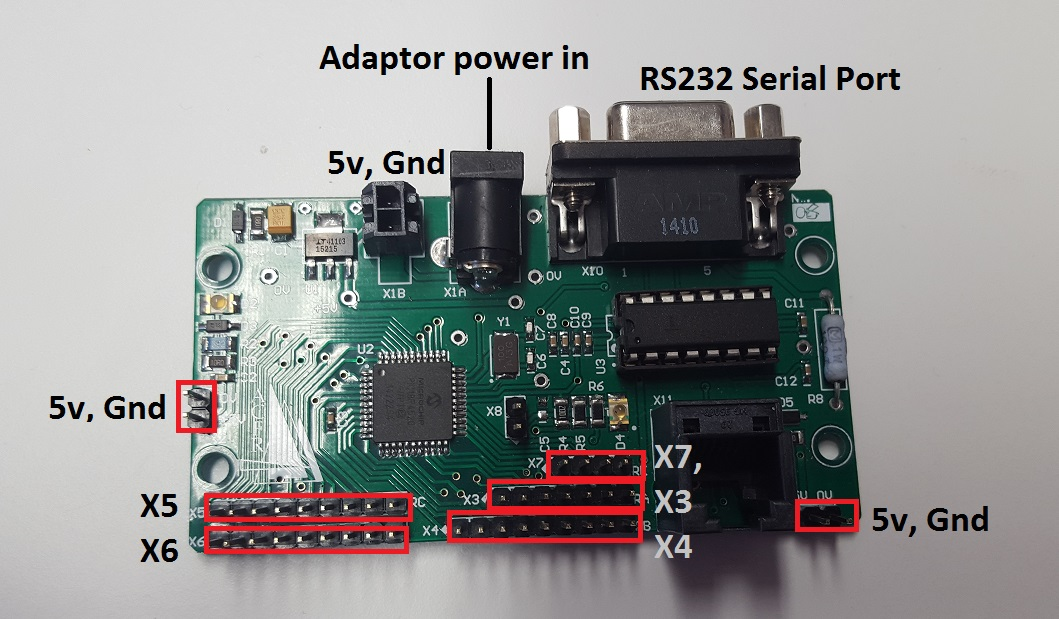
\includegraphics[width=10cm]{pic.png}
      \caption{The PIC18f4520 microcontroller on the minimal board}
      \label{fig:PIC}
  \end{figure}
  \begin{table}
    \centering
      \begin{minipage}{0.45\textwidth}
        \begin{tabular}[b]{|p{7mm}|p{15mm}|}
          \hline \textbf{Pin} & \textbf{Signal}\\
          \hline X3.1 & PortA.0\\
          \hline X3.2 & PortA.1\\
          \hline X3.3 & PortA.2\\
          \hline X3.4 & PortA.3\\
          \hline X3.5 & PortA.4\\
          \hline X3.6 & PortA.5\\
          \hline X3.7 & +0 V   \\
          \hline
        \end{tabular}
        \caption{PORT A connector, X3}
        \vspace{25pt}
      \end{minipage}\hfill
      \begin{minipage}{0.45\textwidth}
        \begin{tabular}[b]{|p{7mm}|p{15mm}|}
          \hline \textbf{Pin} & \textbf{Signal}\\
          \hline X4.1 & PortB.0\\
          \hline X4.2 & PortB.1\\
          \hline X4.3 & PortB.2\\
          \hline X4.4 & PortB.3\\
          \hline X4.5 & PortB.4 (LED)\\
          \hline X4.6 & PortB.5\\
          \hline X4.7 & PortB.6\\
          \hline X4.8 & PortB.7\\
          \hline X4.9 & +0 V\\
          \hline
        \end{tabular}
        \caption{PORT B connector, X4}
      \end{minipage}\hfill
  \end{table}
  \begin{table}
    \flushleft
      \begin{minipage}{0.3\textwidth}
        \begin{tabular}[b]{|p{7mm}|p{15mm}|}
          \hline \textbf{Pin} & \textbf{Signal}\\
          \hline X5.1 & PortC.0\\
          \hline X5.2 & PortC.1\\
          \hline X5.3 & PortC.2\\
          \hline X5.4 & PortC.3\\
          \hline X5.5 & PortC.4\\
          \hline X5.6 & PortC.5\\
          \hline X5.7 & PortC.6\\
          \hline X5.8 & PortC.7\\
          \hline X5.9 & +0 V\\
          \hline
        \end{tabular}
        \caption{PORT C connector, X5}
        \vspace{25pt}
      \end{minipage}\hfill
      \begin{minipage}{0.3\textwidth}
        \begin{tabular}[b]{|p{7mm}|p{15mm}|}
          \hline \textbf{Pin} & \textbf{Signal}\\
          \hline X6.1 & PortD.0\\
          \hline X6.2 & PortD.1\\
          \hline X6.3 & PortD.2\\
          \hline X6.4 & PortD.3\\
          \hline X6.5 & PortD.4\\
          \hline X6.6 & PortD.5\\
          \hline X6.7 & PortD.6\\
          \hline X6.8 & PortD.7\\
          \hline X6.9 & +0 V\\
          \hline
        \end{tabular}
        \caption{PORT D connector, X6}
        \vspace{25pt}
      \end{minipage}\hfill
      \begin{minipage}{0.3\textwidth}
        \begin{tabular}[b]{|p{7mm}|p{15mm}|}
          \hline \textbf{Pin} & \textbf{Signal}\\
          \hline X7.1 & PortE.0\\
          \hline X7.2 & PortE.1\\
          \hline X7.3 & PortE.2\\
          \hline X7.4 & +0 V\\
          \hline
        \end{tabular}
        \caption{PORT E connector, X7}
      \end{minipage}\hfill
  \end{table}

\end{document}
